% !TEX encoding = UTF-8 Unicode

% Beispiel für ein LaTeX-Dokument im Format "seminarvorlage"
\documentclass[ngerman]{seminarvorlage}
% ngerman = Deutsch in neuer Rechtschreibung, alternativ english
\usepackage{babel} % automatische Sprachunterstützung

\usepackage[utf8]{inputenc} % Kodierung der Non-ASCII-Zeichen
\usepackage[T1]{fontenc} % Moderne Fonts, Trennung von Wörtern mit Umlauten
\usepackage{cleveref} % für bequeme Referenzen, siehe \cref unten

\usepackage{embrac}% upright brackets in emphasised text, () and [], empfohlen
\usepackage{pgfplots}
\usepackage{graphicx}

%\usepackage{biblatex}% besser als bibtex, aber dann biber statt bibtex benutzen

\begin{document}

% Unbedingt angeben: Titel, Autoren
% Freiwillig: Adresse, E-Mail
\title{Warum keiner mehr agil arbeiten will}
\numberofauthors{2}
\author{
  \alignauthor Christoph Weber\\
    \email{i22037@hb.dhbw-stuttgart.de}
  \alignauthor Stefan Zimmerer\\
    \email{i22040@hb.dhbw-stuttgart.de}
}

\maketitle% Titelangaben produzieren, aber kein Inhaltsverzeichnis, \tableofcontents funktioniert nicht!
\newpage

\abstract{
}

\keywords{.}

% Section-Überschriften werden automatisch in GROSSBUCHSTABEN gesetzt
\section{Einleitung}

In einer sich rasant wandelnden Welt sind agile Methoden für Unternehmen unverzichtbar geworden.\\
Technologische Fortschritte in Bereichen wie Robotik, Biotechnologie oder künstlicher Intelligenz schaffen schnell neue Möglichkeiten und machen deren Komplexität kaum vorhersehbar. Klimaveränderungen und deren Folgen wie Wassermangel oder extreme Wetterereignisse beeinflussen Logistik und Investitionsentscheidungen. Zudem können neue Zollvorschriften lukrative Geschäftsmodelle von einem Tag auf den anderen zunichtemachen.\\
Diese Dinge führen zu einer Schnelllebigkeit, wodurch es Unternehmen schwerfällt, mit klassischen Methoden und starren Geschäftsmodellen ihre Marktposition zu halten. Daher mussten neue Arbeitsweisen gefunden werden, um sich kontinuierlich und schnell an Veränderungen anpassen zu können.\\
Neben diesen externen Faktoren gibt es auch noch interne Gründe für die Einführung neuer Arbeitsweisen.
Ein wesentlicher interner Treiber ist der Wertewandel im Arbeitsleben. Arbeitnehmer haben den Wunsch eigenverantwortlich Aufgaben zu übernehmen und für den Innovationserfolg des Unternehmens beizutragen.\\
 Agile Methoden wurden daher entwickelt, um sowohl den äußeren Anforderungen als auch den veränderten Erwartungen ihrer Mitarbeitenden gerecht zu werden.%quelle beide bücher

Aktuell werden agile Arbeitsweisen zunehmend hinterfragt und teilweise als ineffektiv und unattraktiv wahrgenommen.\\
Das Ziel dieser Arbeit ist es, die Gründe für diese negative Wahrnehmung zu untersuchen und zu erläutern, warum immer weniger Mitarbeitende bereit sind, agile Methoden anzuwenden. Es wird dabei auf die unterschiedlichen Faktoren eingegangen, welche zur Ablehnung im Umgang mit agilen Methoden führen. Anschließend werden die Auswirkungen des Widerstands gegen agiles Arbeiten erläutert. Abschließend werden Lösungsvorschläge zur Verbesserung der Wahrnehmung und Effizienz von agilen Arbeitsmethoden vorgestellt.



% Jede Section am besten mit einem Kommentar hier im Quelltext markieren
\section{Grundlagen}
\subsection{Was Agilität bedeutet}
Das Thema Agilität und agile Methoden reichen bis in die 1950er Jahre zurück. Damals ist IBM beim Mercury-Projekt der NASA in der Softwareentwicklung inkrementell vorgegangen, die Software wurde also durch kleinste Iterationen kontinuierlich verbessert. Seit 1980 wurden agile Modelle wie Spiral oder Extreme Programming(XP) verwendet.\\
Dies zeigt, dass agile Methoden nicht neu sind und aus verschiedenen Disziplinen geprägt wurde, auch wenn häufig der Eindruck erweckt wird, dass Agilität erst seit dem Agilen Manifest im Jahr 2001 existiert.\\\\%agilität was ist das
Das Agile Manifest wurde von 17 Softwareentwicklern erstellt, um die agile Softwareentwicklung zu leiten. Mittlerweile ist das Agile Manifest auch außerhalb der Softwareentwicklung sehr bekannt.
Das Agile Manifest enthält vier zentrale Werte, wobei jeder Wert durch jeweils zwei Wertepaare abgebildet wird . Dabei wird das erste Wertepaar höher geschätzt als das Zweite. Das bedeutet aber nicht, dass die zweiten Wertepaare unwichtig sind. Im Folgenden werden die vier Grundwerte beschrieben und erläutert.

\textbf{Individuen und Interaktion} mehr als Prozesse und Werkzeuge\\
Der Fokus liegt auf den Menschen und der Zusammenarbeit untereinander. Ein persönliches Gespräch ist dabei wertvoller als ein gut dokumentierter Prozess. Dies lässt sich fördern, indem alle Projektmitglieder im selben Raum sitzen.

\textbf{Funktionierende Software} mehr als Umfasssende Dokumentation\\
Der Schwerpunkt liegt auf der Erstellung von funktionierender Software, weil diese der Mehrwert liefert. Dokumentation soll dabei aber nicht abgeschafft werden, sondern unterstützend eingesetzt werden.

\textbf{Zusammenarbeit mit dem Kunden} mehr als Vertragsverhandlung\\
Eine gute Zusammenarbeit mit dem Kunden ist wichtiger als ein formaler und wasserdichter Vertrag, weil der Kunde durch seine Bedürfnisse ein Teil des Prozesses ist. Ein Vertrag vor Projektbeginn ist nicht in der Lage, alle Situationen im Voraus zu berücksichtigen. Durch eine gemeinsame Abstimmung können Änderungen während der Umsetzung effektiv und gewinnbringend eingeführt werden.

\textbf{Reagieren auf Veränderungen} mehr als das Befolgen eines Plans\\
Ein Plan kann nur so gut sein, wie der Wissenstand zu diesem Zeitpunkt es erlaubt. Da sich Wissen und Rahmenbedingungen kontinuierlich weiterentwickeln, ist es wichtig, auf Veränderungen reagieren zu können. Pläne sollen nicht abgeschafft werden, sollten bei Veränderungen jedoch angepasst werden können.\\

\subsection{Unterschied zur klassischen Arbeitsweise}
Die klassischen und agilen Methoden unterscheiden sich grundlegend in ihrer Herangehensweise an Projekten. Klassische Modelle wie das Wasserfallmodell basieren auf klar strukturierten Vorgehensweisen, während sich agile Methoden durch Flexibilität und iterative Prozesse auszeichnen.\cite{Ant.}\\

\begin{figure}[h]
\centering
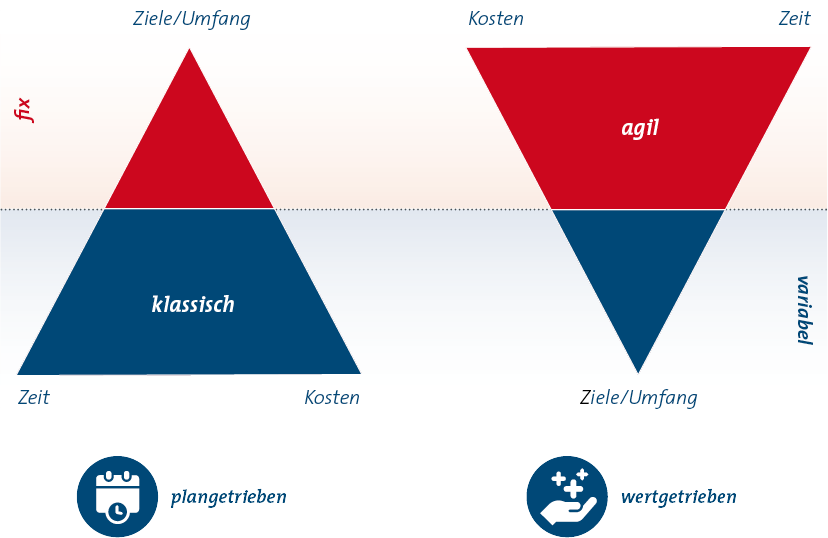
\includegraphics[scale=.5]{"images/klassisch_agil.png"}
\caption{Unterschied klassische vs agile Planung}
\label{agil}
\cite{Consileon.2021}
\end{figure}

In \autoref{agil} ist der Vergleich zwischen der klassischen Planung und der agilen Planung zu sehen. Die Grafik verdeutlicht die entgegengesetzten Prioritäten und Flexibilität der beiden Ansätze.\\ Bei der klassischen Planung sind die Ziele fix, also unveränderlich. Zeit und Kosten sind dagegen variabel und können angepasst werden, um die Ziele zu erreichen. Bei der agilen Planung hingegen sind Kosten und Zeit fix, während die Ziele variabel sind und an Zeit und Kosten angepasst werden.\\  Der klassische Ansatz ist plangetrieben, dabei liegt der Fokus auf der exakten Umsetzung der festgelegten Pläne, unabhängig von Änderungen. Der agile Ansatz ist wertgetrieben, der Fokus liegt auf der Maximierung des Wertes für den Kunden, auch bei Anpassungen an den ursprünglich geplanten Zielen.

Die Auswahl zwischen klassischem oder agilem Projektmanagement hängt von verschiedenen Faktoren ab. Bei klaren Anforderungen und langfristigen Planungen bieten sich klassische Ansätze an. Agile Ansätze bieten sich an, wenn Flexibilität, schnelles Feedback, iterative Verbesserungen und Kundenorientierung im Mittelpunkt stehen.\\ Letztendlich bieten beide Methoden Vor- und Nachteile, die Entscheidung sollte auf den spezifischen Projektanforderungen basieren.

\subsection {Agile Methoden}
\subsubsection{Scrum}
Die am weitesten verbreitete agile Arbeitsmethode ist Scrum. Scrum ist ein Rahmenmodell, damit individuelle Rahmenbedingungen berücksichtigt werden können. Scrum ist einfach und besteht aus wenigen Regeln. Es besteht aus drei Rollen, vier Events und drei Artefakten.\cite{Gaida.2021, Simschek.2022}\\\\
In Scrum gibt es zeitlich begrenzte Ereignisse, die Events. Der Sprint bildet das Herzstück von Scrum. Er ist ein klar begrenzter Zeitraum zwischen zwei bis vier Wochen, in dem ein fertiges, nutzbares Produktinkrement erstellt wird. Im Folgenden werden die vier Events vorgestellt, die ein Sprint umfasst.\\ Im \textbf{Sprint Planning} findet die Planung für den nächsten Sprint statt, also welche Anforderungen umgesetzt werden sollen. Das \textbf{Sprint Review} findet am Ende eines Sprints statt. Dabei wird das Arbeitsergebnis erfasst. Die \textbf{Sprint Retrospektive} findet nach dem Sprint Review und vor dem nächsten Sprint Planning statt. Dabei analysiert das Scrum Team den Ablauf des letzten Sprints, um Verbesserungsmöglichkeiten für den nächsten Sprint zu identifizieren und umzusetzen. Das \textbf{Daily Scrum} ist ein tägliches 15-minütiges Meeting, um die Fortschritte und Hindernisse der Arbeit zu besprechen.\\\\
Scrum besteht aus den Rollen \textbf{Product Owner}, \textbf{Scrum Master} und \textbf{Entwicklungsteam}. Der Product Owner ist für die Priorisierung der Aufgaben verantworlich. Basierend auf den Kundenanforderungen entscheidet er, was im nächsten Sprint umgesetzt werden soll. Der Scrum Master unterstützt das Entwicklungsteam, indem er allen Beteiligten hilft, Scrum zu verstehen und umzusetzen. Der Scrum Master moderiert die Events. Das Entwicklungsteam erledigt die eigentliche Arbeit und ist selbstorganisiert. Außerdem ist das Entwicklungsteam dafür verantwortlich, dass am Ende eines Sprints ein fertiges Inkrement übergeben werden kann.\cite{Mucke.2024}\\\\
Die Artefakte bei Scrum liefern Informationen zu Arbeit und Fortschritt und sind so definiert, dass sie Transparenz bieten, sowie Möglichkeiten zur Überprüfung und Anpassung erlauben.\\ Das \textbf{Produkt Backlog} enthält alle Aufgaben und Anforderungen eines Produkts und wird vom Product Owner verantwortet. Das Product Backlog ist nie final, weil bei der Entwicklung des Produkts neue Anforderungen, Verbesserungen oder Fehler bekannt werden, die bearbeitet werden müssen. Das \textbf{Sprint Backlog} enthält eine Teilmenge der Aufgaben des Product Backlogs. Diese Aufgaben sollen innerhalb dieses Sprints umgesetzt werden.\\ Das \textbf{Inkrement} ist das Ergebnis der im Sprint umgesetzten Arbeit, welches die zuvor erstellten Inkremente erweitert.\\\\
Scrum ist auf kleine Teamgrößen ausgelegt. Das Scrum Team ist klein genug, um flexibel zu bleiben, aber gleichzeitig groß genug, um innerhalb eines Sprints bedeutsame Arbeit zu leisten. In der Regel besteht es aus zehn Personen oder weniger.\cite{Mucke.2024}\\
Ein Merkmal von Scrum ist die klare Abgrenzung der Verantwortlichkeiten. Außenstehende können Einfluss auf das Projekt nehmen, indem sie ihre Änderungswünsche dem Product Owner mitteilen. Es werden innerhalb dieses Sprints aber keine Änderungen an den Anforderungen für diesen Zeitraum vorgenommen, weil das das Entwicklungsteam stören würde. Der Product Owner nimmt die Anforderungen in das Product Backlog auf, welche dann in späteren Sprints bearbeitet werden.\cite{Gluck.2022}
\newpage
\subsubsection{Kanban}
Kanban ist eine agile Projektmanagementmethode, die heutzutage in der Softwareentwicklung verwendet wird. Ursprünglich wurde Kanban von einem Toyota-Ingenieur entwickelt, um das Produktionssytem von Toyota zu verbessern. Dabei orientierte man sich an der tatsächlichen Nachfrage, anstatt wie zuvor Produkte auf Grundlage geschätzter Bedarfszahlen zu produzieren.\cite{Simschek.2022}

Das zentrale Element von Kanban ist das Kanban Board. Dieses ist eine Projekttafel, die aus Spalten besteht. Die Spalten repräsentieren die verschiedenen Phasen eines Arbeitsprozesses. Einfache Kanban Boards haben Spalten wie \glqq To-Do \grqq\: , \glqq In Arbeit \grqq\: und \glqq Erledigt \grqq\: . Die Anzahl der Spalten kann flexibel an die Anforderungen der Produktion angepasst werden.  In der Softwareentwicklung können beispielsweise zusätzliche Spalten wie \glqq In Testung \grqq\: oder \glqq Blockiert\grqq\: integriert werden. Jede Aufgabe wird als visuelle Karte dargestellt, die zwischen den Spalten verschoben werden kann. Beim Anlegen einer Aufgabe wird die Karte in der Spalte "To Do" platziert und einem oder mehreren Beteiligten zugewiesen, die Karte bewegt sich Schritt-für-Schritt nach rechts bis die Aufgabe erledigt ist.\cite{Asana.2024}


In diesem Abschnitt werden sechs Praktiken vorgestellt, welche beachtet werden sollten, um die Vorteile von Kanban nutzen zu können.\cite{Refa.}
\begin{enumerate}
\item Alle Vorgehensweisen müssen transparent kommuniziert werden, damit alle Beteiligten sie verstehen und umsetzen können.
\item Die Anzahl der Karten auf dem Kanban Board muss überschaubar sein.
\item Es müssen immer Karten in der Spalte \glqq In Arbeit\grqq\: vorhanden sein, also immer etwas bearbeitet werden.
\item Alle Kanban Prozesse sollen immer wieder hinterfragt und analysiert werden, um unproduktive Vorgehensweisen aufzudecken und zu beseitigen, um die Effizienz zu erhöhen.
\item Vorgesetzte müssen die Beteiligten so führen, dass sich diese für das Aufrechterhalten des Workflows verantwortlich fühlen und sich für die Optimierung von Abläufen einsetzen.
\item Die grafische Darstellung von Abläufen hilft, Prozesse besser zu verstehen und mögliche Lösungswege aufzuzeigen.
\end{enumerate}

Kanban ermöglicht durch das Kanban Board eine Transparenz, jeder im Team weiß, wer gerade woran arbeitet und wie der Stand der Aufgaben ist. Außerdem hilft das Kanban Board dabei, den Überblick zu behalten und somit auch Engpässe aufzuspüren. Ein weiterer Vorteil ist die flexible Anpassung an die Kundenbedürfnisse, was die Kundenzufriedenheit erhöht. Die einzelnen Bedürfnisse, sei es die Entwicklung eines neuen Produkts oder eine Änderung, werden nach den Anforderungen des Kunden erstellt und als neue Karte auf dem Kanban-Board hinzugefügt.\\\\\\
\subsubsection{Vorteile von agilen Arbeitsweisen}
Der entscheidende Vorteil in der Agilität liegt in der Anpassungs- und Reaktionsfähigkeit. Bei der klassischen Arbeitsweise wird ein Projekt am Anfang so detailliert wie möglich durchgeplant. Dieser Ansatz ist sehr aufwendig und benötigt viele Ressourcen. Das Problem dabei ist, dass bei auftretenden Änderungen oder unerwarteten Problemen eine Umorganisierung der Pläne schwierig ist oder in manchen Fällen gar nicht möglich ist.\\
Bei der agilen Arbeitsweise wird zunächst grob geplant und der Detailgrad immer erst bei Bedarf erhöht. Statt alles am Anfang festzulegen, wird immer nur das geplant, was aktuell absehbar ist. Dadurch wird verhindert, dass unnötig Zeit und Ressourcen in Pläne investiert werden, die später sowieso wieder überarbeitet oder verworfen werden müssen.\cite{Theobald.2021}

Ein weiterer Vorteil ist die hohe Kundenorientierung. Da bei agilen Methoden bereits frühzeitig ein funktionsfähiges Produkt vorhanden ist, kann für dieses Feedback vom Kunden eingeholt werden. Dabei können dem Kunden möglicherweise Dinge auffallen, die er sich anders vorgestellt hat. Durch die Anpassungsfähigkeit der Agilität können die Teams flexibel auf diese veränderten Kundenbedürfnisse reagieren. Dadurch wird die Kundenzufriedenheit gesteigert, was dem Unternehmen einen Wettbewerbsvorteil verschafft.\cite{Theobald.2021,facebook.2024}

Außerdem fördert Agilität Innovation und Kreativität. Dafür gibt es mehrere Gründe. Einerseits arbeiten in den Teams oft Menschen mit unterschiedlichen Fähigkeiten und Mentalitäten zusammen. Dadurch werden Probleme von unterschiedlichen Blickwinkeln betrachtet, wodurch leichter Lösungen gefunden werden können.  Ein weiterer Faktor ist die geförderte Eigenverantwortung. Mitarbeiter haben die Freiheit, Dinge anders handzuhaben und potenzielle Verbesserungen einzubringen. Dafür ist eine entsprechende Vertrauens- und Fehlerkultur wichtig, damit Mitarbeiter bestärkt werden, ihre Verbesserungsideen einzubringen. \cite{Theobald.2021}

Die größere Verantwortung und die Freiheit, direkt auf den Projekterfolg einzuwirken, kann die Motivation der Mitarbeitenden erhöhen. Gleichzeitig wirkt sich die selbstorganisierte Arbeitsweise positiv auf die Arbeitsatmosphäre aus, da Stress vermieden wird, der durch starre Hierarchien verursacht wird. Außerdem führen die kurzen Planungsintervalle und die Unterteilung der Arbeit in kleine Aufgabenpakete zu mehreren erreichbaren Zielen, wodurch während eines Projekts mehrere Erfolgserlebnisse entstehen.\cite{Theobald.2021}

Unternehmen, die agile Arbeitsweisen verwenden, werden von jungen Bewerbern als moderne und attraktive Arbeitgeber wahrgenommen. Durch den Einsatz von agilen Methoden wird potenziellen Mitarbeitern signalisi
ert, dass ihnen Werte wie Autonomie und Zusammenarbeit wichtig sind.\cite{personio.2024}

\newpage
\section{Gründe für das Scheitern mit agilen Methoden}

Obwohl agile Methoden wie Scrum und Kanban viele Vorteile bieten, scheitern deren Implementierungen in der Praxis häufig aus verschiedenen Gründen. \\

\begin{figure}[ht]
    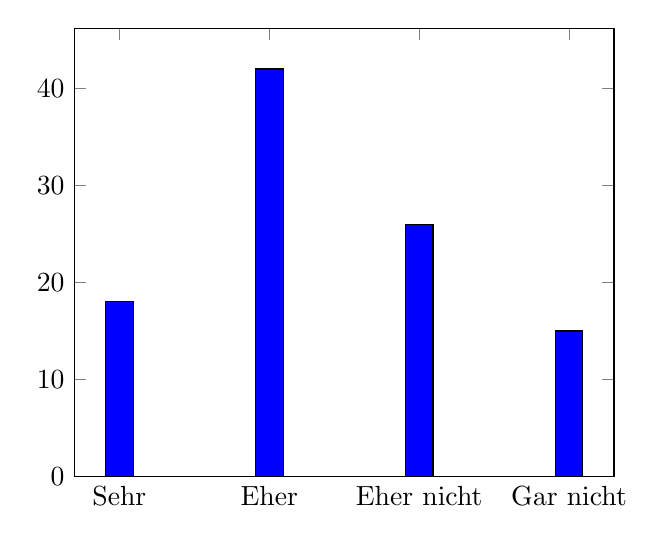
\begin{tikzpicture}
     	 \begin{axis}[
	            symbolic x coords={Sehr, Eher, Eher nicht, Gar nicht},
	            xtick=data,
		  ymin=0
	          ]
	            \addplot[ybar,fill=blue] coordinates {
	                (Sehr,   18)
	                (Eher,  42)
	                (Eher nicht,   26)
		      (Gar nicht, 15)
	            };
       	\end{axis}
    \end{tikzpicture}
    \label{umfrage_}
    \caption{Umfrage zur Zufriedenheit von Agilität}
    %\cite{StateofAgil2023}
\end{figure}

In Abbildung 2 sind die Ergebnisse der Umfrage vom State of Agile Report von 2023 abgebildet. Es geht dabei um die Zufriedenheit von Agilität. Dabei sind 18\% der Befragten sehr zufrieden und 42\% eher zufrieden, was zusammen 60\% zufriedene Teilnehmer ergibt. Im Vergleich zum Vorjahr, in dem noch 72\% zufrieden waren, stellt dies einen Rückgang dar. Außerdem sind 15\% gar nicht zufrieden, was ein deutlicher Anstieg im Vergleich zu den 6\% des Vorjahres ist. Nun stellt sich die Frage, warum die Zufriedenheit von Agilität weniger geworden ist.

Einer der Hauptfaktoren ist der Widerstand gegen Veränderungen, insbesondere in etablierten Organisationsstrukturen, die auf hierarchischen Entscheidungsprozessen basieren. 
Zudem fehlt es oft an ausreichendem Verständnis der agilen Prinzipien und deren konsequenter Anwendung, was zu einer fehlerhaften Umsetzung führt. 
Ein weiterer kritischer Punkt ist die unzureichende Unterstützung durch das Management, wodurch die notwendigen Ressourcen oder die notwendige Kultur der Eigenverantwortung und Kollaboration nicht gefördert werden. 
Auch unrealistische Erwartungen, wie die sofortige Verbesserung von Ergebnissen ohne Berücksichtigung der Lernkurve, tragen zum Scheitern bei. Schließlich können fehlende Kommunikation und unklare Zielsetzungen innerhalb des Teams die Effizienz und den Erfolg agiler Methoden erheblich beeinträchtigen.

\subsection{Fake Agile: Falsche Umsetzung und ihre Folgen}

Agiles Arbeiten verspricht Flexibilität, Anpassungsfähigkeit und Kundenzentrierung. Doch diese Prinzipien können bei falscher Umsetzung verwässert oder sogar ins Gegenteil verkehrt werden – ein Phänomen, das als \textit{Fake Agile} bezeichnet wird. Analog zu \glqq Fake News\grqq{} handelt es sich hierbei um Ansätze, die zwar den Anschein agiler Praktiken erwecken, aber weder deren Kern noch deren Prinzipien verstehen und umsetzen. \textit{Fake Agile} zeigt sich häufig in Form von Cargo-Kult-Methoden, bei denen äußere Merkmale agiler Methoden nachgeahmt werden, ohne die zugrunde liegende Philosophie zu adaptieren.

Ein prägnantes Beispiel ist das Konzept des \textit{Cargo Cult Science}, wie es von dem Physiker Richard Feynman beschrieben wurde. Hier wird der äußere Schein – beispielsweise durch Stand-up-Meetings oder Scrum-Boards – nachgebildet, ohne die grundlegenden Werte wie iteratives Lernen, Transparenz und Teamverantwortung zu verstehen. Diese Oberflächenorientierung führt zu ineffizienten Prozessen, die wenig zur Wertschöpfung beitragen und oft nur Frustration bei den Beteiligten erzeugen.

Häufig scheitern solche Implementierungen an Missverständnissen: Manche Unternehmen erwarten von agilen Methoden eine universelle Lösung aller Probleme. Andere wiederum übertragen die Verantwortung unreflektiert auf Teams, ohne die notwendige Struktur, Kommunikation oder Führungsunterstützung bereitzustellen. Nicht selten entsteht dabei ein organisatorischer Wildwuchs, der mehr Chaos als Innovation fördert. In extremen Fällen können sich isolierte Teamstrukturen entwickeln, die sich gegen die Gesamtorganisation abschotten und gefährliche Dynamiken fördern.

Um \textit{Fake Agile} zu vermeiden, bedarf es einer kritischen Reflexion über die eigenen Zielsetzungen, ein tiefes Verständnis der agilen Prinzipien und eine kontinuierliche Anpassung auf Grundlage empirischer Erkenntnisse. Unternehmen sollten wissenschaftliche Methoden wie Datenanalysen und Simulationen nutzen, um die Effektivität ihrer agilen Maßnahmen regelmäßig zu überprüfen. Nur so kann aus agiler Methodik eine nachhaltige und sinnvolle Praxis werden, die tatsächlich zur Resilienz und Wettbewerbsfähigkeit eines Unternehmens beiträgt.
\cite{Mucke.2024}

\subsection{Kommerzialisierung der Agilität}

Ein wesentlicher Grund für das Scheitern mit agilen Methoden ist die zunehmende Kommerzialisierung der Agilität, auch bekannt als „agil-industrieller Komplex“. Dieser Begriff beschreibt die Geschäftsmacherei rund um agile Methoden, insbesondere Scrum. Organisationen wie Scrum.org oder die Scrum Alliance haben ein profitables Geschäftsmodell entwickelt, das auf Zertifikaten, Workshops und Train-the-Trainer-Programmen basiert. Dabei wird nicht die Förderung agiler Prinzipien in den Fokus gestellt, sondern der Umsatz durch vermeintlich essenzielle Schulungen und Zertifikate.

Zertifizierungen nehmen dabei eine zentrale Rolle ein. Sie vermitteln den Eindruck, dass nur zertifizierte Fachkräfte agile Methoden erfolgreich anwenden können. Dies führt jedoch oft zu einem bürokratischen Formalismus, der die tatsächlichen Werte der Agilität verdrängt. Zwar ändern sich die Inhalte solcher Zertifikate selten, doch deren regelmäßige Erneuerung wird kostenpflichtig verlangt, was eine Scheinwelt schafft, in der formale Nachweise über tatsächliches Verständnis und Kompetenz gestellt werden.

Ein weiteres Problem ist die Vermarktung agiler Methoden als universelles Allheilmittel. Scrum und ähnliche Ansätze werden von Coaches und Beratungsunternehmen oft als Lösungen für sämtliche organisatorischen Herausforderungen angepriesen. Diese Darstellung verkennt jedoch, dass Agilität nur dann erfolgreich sein kann, wenn sie auf die spezifischen Bedürfnisse und Gegebenheiten eines Unternehmens abgestimmt wird. Die daraus resultierenden überzogenen Erwartungen führen bei Misserfolgen häufig zu Frustration und wachsender Skepsis gegenüber agilen Ansätzen.

Die Kommerzialisierung hat dazu geführt, dass sich viele Unternehmen stärker auf die äußeren Symbole und Formalitäten agiler Methoden konzentrieren als auf deren eigentliche Umsetzung. Statt in die Entwicklung einer agilen Unternehmenskultur oder die Verbesserung der Zusammenarbeit zu investieren, wird oft unverhältnismäßig viel Geld für Zertifikate und externe Schulungen ausgegeben. Diese oberflächliche Implementierung lässt die grundlegenden Werte wie Iteration, Selbstorganisation und Kundenorientierung in den Hintergrund treten.

Um der Kommerzialisierungsfalle zu entkommen, sollten Unternehmen kritisch mit den Angeboten des Marktes umgehen und sich auf die tatsächlichen Bedürfnisse ihrer Organisation fokussieren. Es gilt, die Eigenverantwortung der Teams zu stärken und agile Prinzipien praxisnah umzusetzen, anstatt auf formale Nachweise zu vertrauen. Zudem ist es wichtig, sich nicht von Trends oder unrealistischen Versprechungen leiten zu lassen, sondern Agilität als Werkzeug zu verstehen, das kontinuierliche Anpassung und kritische Reflexion erfordert.

Die Kommerzialisierung zeigt, wie leicht eine sinnvolle Methodik durch den Fokus auf Profit und Formalitäten entwertet werden kann. Nur durch eine Rückbesinnung auf die grundlegenden Werte und eine maßvolle, pragmatische Anwendung kann Agilität ihren ursprünglichen Zweck erfüllen und nachhaltig zur Wettbewerbsfähigkeit von Unternehmen beitragen.
\cite{heise.2024}

\subsection{Widerstand gegen Veränderung und Kulturkonflikte}
Der Widerstand gegen Veränderung ist ein tief verwurzeltes Problem der Menschheit. Veränderungen erzeugen Unsicherheit und Angst. Das liegt daran, weil die Führungskräfte und Mitarbeiter den Verlust von Stabilität, Macht oder klaren Verantwortlichkeiten fürchten. In einer traditionellen Unternehmensstruktur mit festen Hierarchien und Prozessen, werden agile Arbeitsmethoden oft als Bedrohung angesehen.\cite{Frischherz.2024}

Dadurch entsteht Widerstand, den es in verschiedenen Formen gibt: passiver Widerstand, aktiver Widerstand oder Widerstand von der Führugsposition aus.\\ Passiver Widerstand tritt auf, wenn die Mitarbeiter sich an alte Prozesse und Arbeitsweisen klammern, obwohl neue Methoden einegführt wurden. Dadurch wird die Implementierung von neuen Methoden verzögert oder vollständig scheitert.\\ Aktiver Widerstand ist die offene Form der Ablehnung, wobei Mitarbeiter ihre Unzufriedenheit lautstark äußern. Dadurch kann auch die Effektivität der eingeführten Veränderungen beeinträchtigt werden. \\Beim Widerstand aus der Führungsposition blockieren Manager und Führungskräfte die Einführung agiler Methoden, um ihre Machtpposition zu sichern. Sie befürchten, dass die neuen Methoden ihre Rolle überflüssig machen könnte.

Die Einführung von Agilität ist aufgrund von Kulturkonflikten oft nicht möglich. Agile Prinzipien setzen auf Transparenz, Vertrauen und Zusammenarbeit. Traditionelle Unternehmenskulturen hingegen setzen auf Kontrolle, Wettbewerb und Silodenken. Silodenken beschreibt eine Situation im Unternehmen, bei der Abteilungen oder Teams isoliert voneinander arbeiten und kaum über Abteilungen hinweg miteinander kommunizieren. Andere Abteilungen werden dabei oft als irrelevant oder sogar inkompetent abgetan.\\ Je stärker sich die bestehenden Werte und Prinzipien von den agilen Prinzipien unterscheiden, desto schwieriger ist die Transformation. Dies führt oft dazu, dass die gewünschten Ergebnisse ausbleiben oder die Situation sich sogar verschlechtert.\cite{Natsiopoulou.,tractionwise.2023}

Ein konkreter Kulturkonflikt sind die Entscheidungen. In traditionellen Unternehmensstrukturen werden die Entscheidungen von den Führungskräften getroffen, während bei agilen Arbeitsweisen schnell auf Team-Ebene entschieden wird. Das führt zu einem Widerspruch. Das agile Team fühlt sich ausgebremst, wenn nur Vorgesetzte Entscheidungen treffen, während Führungskräfte den Eindruck haben, die Kontrolle zu verlieren, wenn die Entscheidungen vom Team getroffen werden.\\
Ein weiterer Konfliktpunkt ist die Fehlerkultur, also der Umgang mit Fehlern. Agilität betont das Lernen aus Fehlern und diese als Teil des Prozesses zu akzeptieren, während traditionelle Kulturen Fehler als Misserfolg ansehen.\cite{wavestone.2024}

\subsection{Führungskräfte}
Wie im vorherigen Grund schon angeschnitten, sind Führungskräfte ein weiterer Grund für den Erfolg oder Nichterfolg von Agilität. Wenn Führungskräfte den Mehrwert von agilem Arbeiten nicht erkennen und deshalb die Transformation nicht aktiv unterstützen, wird selbst ein hochmotiviertes Team kein Erfolg haben. Das Problem ist dabei, dass die Führungskräfte nicht voll dahinterstehen und bei Unsicherheiten oder Schwierigkeiten wieder auf alte Gewohnheiten zurückgegriffen wird. Dadurch werden die agilen Bemühungen untergraben und widersprüchliche Signale an die Mitarbeiter gesendet.\\
Es macht eine gute Führungskraft aus, sich auf Veränderungen einzulassen und eine aktive Rolle im Prozess der Transformation einzunehmen, sodass auch die Mitarbeiter an diese Veränderung glauben.\\\\
Bei der agilen Führung haben Führungskräfte eine andere Rolle als bei einer tradionellen Unternehmenskultur. Anstatt zu dirigieren und zu kontrollieren sollten sie eine eher beratende Rolle einnehmen. Dabei sollten Führungskräfte dem Entwicklungsteam als Begleiter und Coaches zur Verfügung stehen und das Entwicklungsteam die Entscheidungen treffen lassen. Außerdem sollten sie die Stärken der einzelnen Mitarbeiter erkennen und fördern. Somit tragen sie zur Weiterentwicklung der Mitarbeiter bei. Außerdem sollten sie die Mitarbeiter gemäß ihrer Kompetenzen einsetzen.\cite{cleverlance.2024}

Viele Führungskräfte haben Schwierigkeiten, diese Rolle anzunehmen und Verantwortung abzugeben. Sie treffen dann oft selbst entscheidende Entscheidungen. Dadurch hat das Team den Eindruck, nicht ausreichend Vertauen zu bekommen, was zu Demotivation und Frustration führen kann. Mittarbeiter haben das Gefühl, entmachtet zu sein und nur noch Anweisungen auszuführen, anstatt eigenständig Probleme zu lösen und Verantwortung zu übernehmen.

Ein weiteres Hindernis ist die mangelnde Klarheit bezüglich der Ziele und Prioritäen. Agile Methoden wie Scrum oder Kanban erfordern regelmäßige Überprüfungen und Anpassungen der Ziele. Teams benötigen klare Ziele, um effektiv zusammenarbeiten zu können. Wenn Führungskräfte nicht in der Lage sind, Ziele und Prioritäten verständlich zu kommunizieren, führt das zu Ineffizienz, weil die Arbeitsergebnisse nicht den Erwartungen entsprechen und die Anforderungen verfehlen.

\subsection{Produkte}

Ein weiterer Grund für das Scheitern einer agilen Transformation sind die Produkte. Agile Arbeitsweisen wie Scrum oder Kanban haben ihre Vorteile vor allem in der Softwareentwicklung, wo sich die Software laufend verändert und schnelle Anpassungen durch iterative Zyklen möglich sind. Bei physischen Produkten mit langen Entwicklungszyklen stößt Agilität schnell an seine Grenzen\cite{Simons.2021}.\\\\
Hochkomplexe Maschinen, Flugzeuge oder medizinische Geräte sind auf langfristige Planungen, umfangreiche Tests und gesetzliche Anforderungen angewiesen. Diese Produkte können nicht einfach nach einer Iteration in einer unvollständigen Form auf den Markt gebracht werden und dann kontinuierlich verbessert werden. Ein Flugzeug, dass noch nicht alle Funktionen enthält und deshalb noch nicht alle Tests bestanden hat ist ein Sicherheitsrisiko, genau so wie nicht fertiggestellte medizinische Geräte. Für Unternehmen, die solche Produkte herstellen, ist agiles Arbeiten nicht praktikabel.

Außerdem gibt es Branchen, bei denen die Anforderungen an Produkte so starr sind, dass ein iterativer Entwicklungsprozess kaun umsetzbar ist.\\ Ein Beispiel sind sicherheitskritische Systeme in der Automobil- und Raumfahrtindustrie. Hier werden die technischen Spezifikationen am Anfang der Entwicklung festgelegt, weil sie durch gesetzliche oder behördliche Vorgaben definiert werden. Weil bei diesen Produkten präzise Planung und Kontrolle gefordert ist, sind hier klassische Methoden besser als agile Methoden.

Ein weiterer Faktor ist der Produktionsprozess selbst. Software kann einfach aktualisiert und digital verteilt werden. Physische Produkte hingegen sind an Produktionslinien, Materialien und Lieferketten gebunden. Das Ändern der Anforderungen und Umpriorisieren verursacht erhebliche Kosten und kann die Lieferkette beeinträchtigen. Auch in diesem Beispiel macht es keinen Sinn, Agilität einzuführen, weil die erforderliche Flexibilität für agile Methoden nicht gegeben ist.


\section{Auswirkungen}
Die fehlerhafte oder unzureichende Implementierung agiler Methoden kann auf verschiedenen Ebenen gravierende Konsequenzen haben. Diese betreffen die Teamdynamik, die Unternehmensebene und die Arbeitskultur, wobei sie die grundlegenden Ziele agiler Ansätze wie Flexibilität, Effizienz und Innovationskraft gefährden.

\subsection{Auswirkungen auf die Teamdynamik}
Fehler in der Einführung agiler Methoden haben erhebliche Auswirkungen auf die Dynamik innerhalb von Teams. Ein zentrales Problem ist die unklare Kommunikation über die Gründe für die Einführung und den Nutzen agiler Methoden. Dies führt zu Unsicherheiten, Ängsten und Widerständen, etwa aus der Sorge, den eigenen Status zu verlieren oder mit den neuen Prozessen nicht zurechtzukommen.

Zusätzlich fühlen sich Teams häufig überfordert, wenn zentrale Prinzipien wie Selbstorganisation und iterative Anpassung nicht konsequent gelebt werden. Ein formalistischer Ansatz, der Agilität als starres Regelwerk missinterpretiert, verstärkt diese Überforderung und beeinträchtigt die Produktivität.

Viele agile Schulungen tragen ebenfalls zur Frustration bei, da sie stark theoretisch und wenig praxisnah gestaltet sind. Mitarbeitende können das Gelernte häufig nicht auf ihre spezifischen Aufgaben anwenden, was zu Orientierungslosigkeit und einem Gefühl von Inkompetenz führt. Diese Erfahrungen mindern das Vertrauen in agile Methoden und erschweren die erfolgreiche Umsetzung.

Ein weiteres Hindernis ist die unzureichende Integration agiler Teams in die Gesamtorganisation. Isolierte agile Einheiten haben oft nur wenig Kontakt zu anderen Abteilungen, was zu Missverständnissen und Konflikten führt. Unterschiedliche Arbeitsweisen zwischen agilen und nicht-agilen Teams belasten den Zusammenhalt und erschweren die Zusammenarbeit.

Zudem fehlt es in vielen Fällen an Vorbildern auf Führungsebene. Während Teams Flexibilität und Eigenverantwortung leben sollen, halten Führungskräfte häufig an traditionellen Hierarchien fest. Diese Doppelmoral untergräbt das Vertrauen in die agilen Prinzipien und führt zu Frustration innerhalb der Teams.
\cite{moutafis_warum_2019}

\subsection{Auswirkungen auf Unternehmen}
Die fehlerhafte Einführung agiler Methoden führt auf Unternehmensebene häufig dazu, dass die angestrebten Vorteile wie Flexibilität, Effizienz und Innovationskraft ins Gegenteil umschlagen. Anstelle agilerer und wettbewerbsfähigerer Strukturen kämpfen viele Organisationen mit ineffizienten Prozessen, Ressourcenverschwendung und einer sinkenden Wettbewerbsfähigkeit. Dies geschieht oft, weil die agile Transformation ohne eine fundierte strategische Planung oder Anpassung an die spezifischen Bedürfnisse des Unternehmens durchgeführt wird. Das Ergebnis sind eine Flut von Meetings, uneinheitliche Arbeitsweisen und eine mangelnde Abstimmung zwischen Abteilungen. Anstelle der angestrebten Effizienz entstehen bürokratische Hürden, die die Produktivität hemmen und die Mitarbeitenden demotivieren.

Darüber hinaus investieren Unternehmen häufig erhebliche Mittel in Schulungen und Beratungsprojekte, die jedoch wenig praxisorientiert sind und die spezifischen Herausforderungen der Organisation nicht berücksichtigen. Infolgedessen fällt es den Mitarbeitenden schwer, das Erlernte in ihren Arbeitsalltag zu integrieren, was dazu führt, dass die Transformation ins Stocken gerät. Wenn kurzfristige Ergebnisse ausbleiben, verlieren viele Organisationen das Vertrauen in die agile Methodik und kehren zu traditionellen Ansätzen zurück. Dies führt nicht nur zu finanziellen Verlusten, sondern auch zu einer Verfestigung bestehender Strukturen, die einer agilen Weiterentwicklung im Wege stehen.

Ein weiteres Problem ist die fehlende Integration agiler Methoden in die Gesamtstrategie des Unternehmens. Häufig agieren agile Teams isoliert und ohne klare Schnittstellen zu anderen Abteilungen, was zu Missverständnissen und einer mangelnden Abstimmung führt. Zudem wird die Transformation häufig von oben beschlossen, ohne die Mitarbeitenden ausreichend in den Prozess einzubeziehen. Dies verursacht Widerstände und verhindert, dass sich die Mitarbeitenden mit den neuen Prozessen identifizieren.

Ein entscheidendes Hindernis stellt auch das Verhalten der Führungsebene dar. Während von den Mitarbeitenden erwartet wird, agile Prinzipien zu leben, halten viele Führungskräfte an traditionellen hierarchischen Strukturen fest. Diese Inkonsistenz untergräbt die Glaubwürdigkeit der Transformation und schafft eine Kultur des Misstrauens. Zudem wird der Erfolg agiler Projekte oft nach den Maßstäben traditioneller Ansätze bewertet, wodurch Erfolge nicht anerkannt und agile Methoden als ineffizient abgetan werden.

Diese Herausforderungen wirken sich langfristig negativ auf die Wettbewerbsfähigkeit eines Unternehmens aus. Wenn agile Prinzipien nicht effektiv umgesetzt werden, erschwert dies die Anpassung an sich verändernde Marktbedingungen und hemmt Innovationen. Unternehmen, die die Potenziale agiler Arbeitsweisen nicht nutzen, riskieren, den Anschluss an die Konkurrenz zu verlieren und sich langfristig in einer stagnierenden Position wiederzufinden.
\cite{online_chef_2022}

\subsection{Auswirkungen auf die Arbeitskultur}
Die unsachgemäße Einführung agiler Methoden wirkt sich auch negativ auf die Arbeitskultur aus. Fehler in der Umsetzung führen zu einer Abwertung moderner Arbeitsweisen und einer generellen Skepsis gegenüber Veränderungen.

Ein häufiger Effekt ist der Vertrauensverlust in agile Methoden. Wenn diese nur unvollständig oder fehlerhaft umgesetzt werden, können sie ihre Vorteile nicht entfalten. Solche Erfahrungen prägen die Wahrnehmung der Mitarbeitenden und führen häufig dazu, dass agile Ansätze pauschal abgelehnt werden.

Die Rückkehr zu traditionellen Hierarchien ist eine weitere Folge. Scheitert die agile Transformation, verfestigt sich die Überzeugung, dass traditionelle Arbeitsweisen überlegen sind. Dies erstickt Flexibilität und Innovation und führt zu einer Kultur, die Veränderungen scheut.

Schließlich können falsche Ansätze bei der Einführung agiler Methoden zu Demotivation und Konflikten im Team führen. Ohne klare Kommunikation und Zustimmung der Mitarbeitenden entstehen Widerstände, die sowohl die Zusammenarbeit als auch die Produktivität beeinträchtigen.

Langfristig gefährdet die negative Wahrnehmung agiler Methoden die Innovationsfähigkeit der Organisation. Anstelle einer Kultur des Lernens und der kontinuierlichen Verbesserung entsteht eine sicherheitsorientierte Denkweise, die die Weiterentwicklung der Organisation behindert und ihre Wettbewerbsfähigkeit schwächt.
\cite{stawicki_10_2021}

%- Auf die Teamdynamik (Frustration, Demotivation, Konflikte)
%- Auf Unternehmen (Fehlende Effizienz, hohe Kosten, sinkende Wettbewerbsfähigkeit)
%- Auf die Arbeitskultur (Vertrauensverlust in moderne Methoden, Rückkehr zu traditionellen Ansätzen)

\section{Alternativen und Lösungsansätze}
%- Hybride Ansätze

% und schon der letzte Abschnitt
\section{Fazit}
%- Zusammenfassung der wichtigsten Erkenntnisse
%- Kritische Reflexion: Zukunft agiler Arbeitsweisen und ihr Potenzial


% Bibliographie entweder direkt hier eingeben (nur im Notfall)...
%\begin{thebibliography}{9}
%\bibitem{ACM2019}
%ACM.
%\newblock How to classify works using ACM's computing classification system.
%\newblock \url{http://www.acm.org/class/how_to_use.html}.
%
%\bibitem{Ivory2001}
%M.~Y. Ivory and M.~A. Hearst.
%\newblock The state of the art in automating usability evaluation of user
%  interfaces.
%\newblock {\em ACM Comput. Surv.}, 33(4):470--516, 2001.
%
%\end{thebibliography}

% ... oder die Bibliographie mit Hilfe von BibTeX generieren,
% dies ist auf jeden Fall die bessere Lösung und sollte nach
% Möglichkeit immer verwendet werden:
\bibliographystyle{abbrv}
\bibliography{literatur} % Daten aus der Datei literatur.bib verwenden.

\end{document}
